% ======================================================================
% 中文稿 main_zh.tex —— 与英文稿 manuscript/main.tex 同源的中文版本
%
% 用途：英文稿（master）逐段审核定稿后，同步维护的中文对应稿；
%       若英文投稿不顺，可在此基础上改投中文期刊。
% 纪律：英文稿是唯一 master。本文件只收录"已定稿"的段落；
%       未审核的节以【待同步】占位，不自行创作。
%       冻结数字与英文稿逐字一致（见 manuscript/SCIENTIFIC_CHECKSUM_V06.csv）。
% 编译：latexmk -xelatex -outdir=build main_zh.tex  （需 XeLaTeX + ctex）
% 参考文献：暂用 IEEEtran 数字式（与英文稿共用 ../references.bib）；
%       确定目标中文期刊后按其规范换 GB/T 7714（biblatex-gb7714-2015）。
% ======================================================================
\documentclass[zihao=5,a4paper]{ctexart}

\usepackage{amsmath,amssymb}
\usepackage{bm}
\usepackage{graphicx}
\usepackage{booktabs}
\usepackage{cite}
\usepackage[margin=2.4cm]{geometry}
\graphicspath{{../figures/}}

% ---- 与英文稿一致的宏 ----
\DeclareRobustCommand{\Cuk}{\mbox{\'{C}uk}}
\newcommand{\ESR}{\ensuremath{\mathrm{ESR}}}
\newcommand{\TSRLS}{TS-D-RLS}
\newcommand{\TSKF}{TS-SLTVKE}
\newcommand{\TSSRKE}{TS-SRKE}
\newcommand{\alphab}{\bar{\alpha}}
\newcommand{\vect}[1]{\bm{#1}}
\newtheorem{proposition}{命题}
\newtheorem{remark}{注记}

\title{面向\Cuk{}能量传递电容在线C--ESR监测的\\拓扑同步解耦观测与监督重置估计}
\author{（作者信息待定）}
\date{}

\begin{document}

\maketitle

\noindent\textbf{摘要：}
\Cuk{}变换器中的能量传递电容是可靠性关键的功率传递元件，但纹波测量将其容值与等效串联电阻（ESR）耦合在一起。本文提出拓扑同步、方向解耦的观测，在不施加诊断注入的情况下利用$+i_{L1}$与$-i_{L2}$之间的电流换流：对带保护带的边沿窗口内带时间戳的采样进行局部拟合，重构ESR主导的不连续量；状态内电荷积分给出容值主导的观测行。正的有限窗信息下界在有效连续导通模式条件下建立局部可辨识性。在这些观测之上，监督重置Kalman估计器（\TSSRKE{}）在Joseph形式核上叠加预声明的双时间尺度监督器，作用于被接受与被门限拒绝的新息，在健康参数突变后恢复增益而不扰动区间校准。评估覆盖48个盲例、四档噪声与四档时间偏斜，并包含突变阶跃、退化斜坡与TMS320F28379D器件级场景。仿真结果表明：仅采用所提观测（RLS核不变）即可将平均容值误差从$7.0366\%$降至$0.3727\%$；\TSSRKE{}取得$0.3011\%/0.6446\%$的容值/ESR误差与$88.93\%$的联合覆盖率，且在稳态下与其母体逐位一致。容值与ESR突变分别在$1.52$与$0.48$~ms内收敛，而无监督核不能恢复；最差95百分位误差$1.6425\%/2.6109\%$支持所建模DSP约束下的器件级可行性。

\vspace{0.5em}
\noindent\textbf{关键词：}\Cuk{}变换器；电容状态监测；变化检测；能量传递电容；容值估计；等效串联电阻；Kalman滤波；参数辨识；电力电子可靠性

\section{引言}
\label{sec:introduction}

电容器是电力电子变换器中可靠性关键的元件，其健康状态直接影响变换器的可用性\cite{wang2014reliability}。然而，电容器在持续的电应力与热应力作用下会发生退化，由此产生的容值衰减与等效串联电阻（ESR）增长又反过来改变电应力、热损耗与滤波性能；这两个量是电解电容与薄膜电容公认的退化前兆\cite{wang2014reliability,yao2024film}。由于这两个参数在运行中均不可直接测量，人们发展了众多在线监测方法，涵盖纹波分析、注入激励、电路重构、观测器、递推辨识与数据驱动处理\cite{dang2020review,nathan2023review,zhao2021overview}。某一具体方案是否适用，取决于电容器的电路角色以及哪些电气量本来就在测量之列。

\Cuk{}变换器中的能量传递电容不同于直流母线电容或输出滤波电容：它位于主功率传递路径上，交替承载完整的电感电流$+i_{L1}$与$-i_{L2}$。因此每次开关切换都使电容电流在两个带符号的值之间换流，而正常运行本身就以开关频率提供这种双向激励，无需任何诊断性扰动。把这个元件当作异步采样的普通二端电容处理，恰恰丢弃了这一拓扑特有的信息。

现有的C--ESR联合辨识方法都是从其他电路角色切入这一问题的。Hasegawa等\cite{hasegawa2018dclink}通过分离逆变器直流母线中的纹波频率分量来估计母线容值与ESR；然而该分离方法受限于该拓扑的纹波频带。Yao等\cite{yao2015buck}利用PWM信号与输出电压、在无电流传感器条件下辨识buck输出电容的ESR与容值，相关的无传感器方案延续了这一路线\cite{tang2019sensorless}；然而其底层的周期内关系假设了buck输出级的单向滤波电流，无法迁移到电流在每个子区间内都反向的电容上。基于观测器的方案\cite{barbulescu2022observer,barbulescu2023implementation,caiman2024quasionline}通过切换电阻网络获得联合估计；然而它们需要附加放电网络，或只能在准在线区间内监测。Ribeiro等\cite{ribeiro2025inherent,ribeiro2024injection,ribeiro2023wavelet}为中点钳位（NPC）直流母线电容提取固有或注入的频谱特征；然而注入增加损耗，且固有信号映射专属于母线频谱。最新扩展包括无传感器boost~ESR估计、buck电容的优化注入以及大信号C--ESR估计\cite{leong2025boostesr,zhang2025injection,zhang2025largesignal}。经实验验证的母线监测也在持续推进：牵引逆变器的极大似然估计、级联H桥的自适应遗忘递推最小二乘（RLS）、放电轮廓与灰箱瞬态方法、多电平变换器ESR--C方案、以及DSP高效的频谱前兆\cite{wu2025mlrail,wang2024chb,wei2024discharge,zhao2023greybox,deng2020mmc,asoodar2024mmc,sundararajan2020goertzel}；小波/Kalman与RLS/Kalman形式提供了更多估计路线\cite{amaral2024waveletkf,zhang2025haar,reichbach2016rls,chen2018vffrls}。针对\Cuk{}变换器本身，已有分数阶建模、变换器故障诊断、传感器故障检测与预测研究\cite{wang2021fractionalcuk,prathiba2023cuk,ajra2024sensorfault,samie2015prognostic}；然而这些工作没有一个利用传递电容的电流换流来做C--ESR联合辨识。

文献\cite{hasegawa2018dclink,yao2015buck,ribeiro2025inherent,amaral2024waveletkf}的非侵入联合方案与\cite{barbulescu2022observer}的观测器路线是与本文最接近的相关方法；由于各研究的变换器拓扑、传感集合与报告协议互不相同，这一对比只能是分类性的而非数值性的。相对于它们全部，本工作的区别在于利用能量传递电容自身的$+i_{L1}\leftrightarrow-i_{L2}$换流，且仅以端电压、两个电感电流、开关状态与时间戳作为测量量。残余的空白是结构性而非算法性的：尚无已报道的方法把\Cuk{}传递机制本身转化为可实现的辨识信息。

因此，本文提出拓扑同步解耦观测，恰好完成这一转化：在带保护带的边沿前后窗口内对带时间戳的采样做局部拟合，在开关时刻重构ESR主导的端电压不连续量；在单一开关状态内做ESR补偿的电荷平衡，得到容值主导的观测行。在第\ref{sec:results}节的共核因子分解实验中，仅采用所提观测（RLS核保持不变）就把平均容值误差从$7.0366\%$降到$0.3727\%$。在这些观测之上构建拓扑同步监督重置Kalman估计器（\TSSRKE{}），它在健康参数突变后恢复增益，同时保持稳态行为不变。整个设计在48个盲例上评估，覆盖四档噪声与四档时间偏斜，并包含突变阶跃、退化斜坡、闭环调节、轻载与TMS320F28379D器件级仿真场景。

本文的主要贡献如下。
\begin{enumerate}
\item 拓扑同步解耦观测：把正常的\Cuk{}开关序列解释为拓扑诱导的健康激励，并通过时间戳重构的边沿拟合与安全窗电荷平衡，将其转化为ESR主导与容值主导的观测行。
\item 由原始观测对建立的联合有限窗可辨识性，以及所实现顺序流的正的各方向信息下界，均在有效连续导通模式条件下成立。
\item 预声明盲验证协议内的观测--估计器因子分解（48个案例、条件Cram\'er--Rao基准与敏感性分析、TMS320F28379D器件级仿真），证明承载主要精度增益的是观测设计而非估计器复杂度的增加。
\item 监督重置扩展（\TSSRKE{}）：通过作用于被接受\emph{以及}被门限拒绝归一化新息的预声明双时间尺度监督器，在健康参数突变后恢复增益；其组件是经典的，所声称的新颖性仅限于它们在门控拓扑同步观测行上的方向专属构造（见第\ref{sec:srke}节）。
\end{enumerate}

本文其余部分组织如下。第\ref{sec:modeling}节建立能量传递电容的开关模型及其健康特征。第\ref{sec:observations}节给出拓扑同步解耦观测框架。第\ref{sec:identifiability}节建立有限窗可辨识性与信息下界。第\ref{sec:estimators}节给出估计核与监督重置实现。第\ref{sec:protocol}节描述验证方法学。第\ref{sec:results}节报告仿真结果。第\ref{sec:device}节评估TMS320F28379D上的器件级可行性。第\ref{sec:discussion}节讨论适用范围与局限。最后，第\ref{sec:conclusion}节总结全文。

% ======================================================================
% 全部章节与附录已随英文稿逐段审核完成同步（2026-08-28，v0.6.25）。
% 后续英文稿任何改动须同步到本文件对应位置。
% ======================================================================

\section{能量传递电容模型与健康特征}
\label{sec:modeling}

\subsection{拓扑、状态与符号约定}

考虑图~\ref{fig:two_states}(a)所示的经典反相\Cuk{}变换器，工作于连续导通模式（CCM）；表~\ref{tab:notation}汇总了主要符号。状态向量为
\begin{equation}
\vect{x}=\begin{bmatrix}i_1&i_2&v_C&v_o\end{bmatrix}^{\mathsf T},
\label{eq:state_vector}
\end{equation}
其中$i_1=i_{L1}>0$与$i_2=i_{L2}>0$沿各自惯常的电感电流方向，$v_C$是能量传递电容中理想元件的内部电压，$v_o>0$是物理上为负的输出电压的幅值。令$u\in\{0,1\}$表示主开关状态，$u=1$为导通。

传递电容电流为
\begin{equation}
i_C=(1-u)i_1-ui_2,
\label{eq:ic_unified}
\end{equation}
因此，与图~\ref{fig:two_states}(b)、(c)的两个开关拓扑对应，
\begin{equation}
u=0:\ i_C=i_1, \qquad u=1:\ i_C=-i_2.
\label{eq:ic_states}
\end{equation}
式~\eqref{eq:ic_unified}是贯穿本文的拓扑专属重构；只要开关状态与两个电感电流可得，即无需在电容支路中设置专用串联电流传感器。

\subsection{非理想电容端口}

一阶电容模型由理想电容$C$与ESR $r_C$串联构成：
\begin{equation}
v_T=v_C+r_C i_C, \qquad \dot v_C=\frac{i_C}{C},
\label{eq:cap_port}
\end{equation}
其中$v_T$是外部可测的端电压。把$v_T$等同于$v_C$会把ESR压降错误归入理想电容，并使两个健康指标耦合。

为数值调理，固定标称电容$C_b$定义
\begin{equation}
\alphab=\frac{C_b}{C}, \qquad C=\frac{C_b}{\alphab}.
\label{eq:alpha_definition}
\end{equation}
健康参数向量为$\vect{\theta}=[\alphab,r_C]^{\mathsf T}$。

\begin{table}[t]
\caption{主要符号}
\label{tab:notation}
\centering
\begin{tabular}{ll}
\toprule
符号 & 含义 \\
\midrule
$u,D,T_s$ & 开关状态、占空比、开关周期 \\
$i_1,i_2$ & 输入、输出电感电流 \\
$i_C$ & 重构的能量传递电容电流 \\
$v_C,v_T$ & 理想内部电压与实测端电压 \\
$C,C_b$ & 实际电容与固定标称电容 \\
$r_C$ & 测量条件下的电容ESR \\
$\alphab$ & 归一化逆电容，$C_b/C$ \\
$q$ & 被接受窗口内传输的电荷 \\
$I_\Sigma$ & 边沿电流和，$i_1+i_2$ \\
$k_R$ & 训练标定、估计期间保持固定的增益 \\
\bottomrule
\end{tabular}
\end{table}

\subsection{健康范围界定}

容值衰减与ESR增长被作为状态指标处理，而不是剩余寿命预测。由于$r_C$依赖温度、频率、工作点与老化，本方法估计的是指定开关与采集条件下的有效ESR。理论假设：反复出现的有效CCM窗口、辨识窗内参数变化可忽略、以及一阶串联C--ESR模型。参数恒定假设是温和的，因为辨识窗为几十毫秒量级，而磨损性漂移以周至月为尺度演化\cite{wang2014reliability}；第\ref{sec:results}节的突变场景正是对该假设失效的直接检验。等效串联电感（ESL）、振铃、断续导通模式（DCM）与前端非理想性通过安全窗选择、标定、门控或明示局限来处理。

只有逆电容被归一化：$\alphab=C_b/C$无量纲，而$r_C$直接以欧姆估计。分离的标量递推与物理界避免二者数值尺度混杂。预声明的ESR区间为$0.35r_b\le r_C\le2.50r_b$，即$r_b=50$~m$\Omega$时的17.5--125~m$\Omega$。评估全程使用的变换器与辨识参数列于表~\ref{tab:converter_parameters}。

本工作的辨识使用端电压、两个电感电流测量、以及开关状态与同步时间戳；缺少任一电感电流测量的应用在第\ref{sec:discussion}节讨论。下一节把这些测量量转化为解耦的健康信息。

\begin{figure*}[t]
\centering
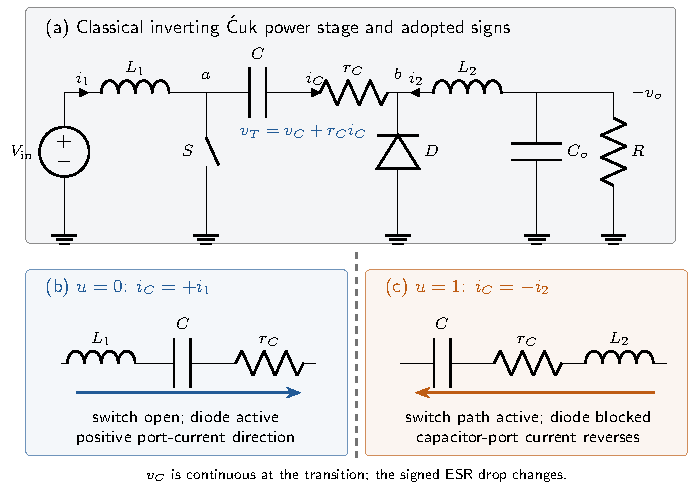
\includegraphics[width=0.98\textwidth]{fig01_cuk_topology.pdf}
\caption{经典反相\Cuk{}变换器与所采用的电流/电压符号约定：(a)~完整功率级；(b)~$u=0$拓扑，$i_C=+i_1$；(c)~$u=1$拓扑，$i_C=-i_2$。理想电容电压$v_C$在切换处连续，而端电压$v_T=v_C+r_Ci_C$含有ESR阶跃。}
\label{fig:two_states}
\end{figure*}

\begin{table}[t]
\caption{变换器与辨识参数}
\label{tab:converter_parameters}
\centering
\begin{tabular}{p{2.2cm}p{4.6cm}}
\toprule
项目 & 取值 \\
\midrule
输入电压 & $V_{\mathrm{in}}=24$~V标称；盲例范围$19.2/24/28.8$~V \\
占空比 & $D=0.40$标称；盲例范围$0.30/0.40/0.55/0.65$ \\
开关频率 & $f_s=50$~kHz（$T_s=20~\mu$s） \\
电感 & $L_1=L_2=500~\mu$H \\
电容 & $C_b=100~\mu$F；$C_o=470~\mu$F \\
标称ESR/负载 & $r_b=50$~m$\Omega$；$R=10~\Omega$ \\
主递推 & $\lambda=0.9975$；$P_0=1000$ \\
边沿标定 & $k_R=0.9772$；训练标定标称值；评估中使用逐例标定值 \\
C电荷窗 & $T_{w,C}=2.0~\mu$s \\
ESR边沿拟合窗 & F28379D实现中$T_{w,R}=2.2~\mu$s \\
健康报告 & 每1024周期（$=20.48$~ms）对外报告一次 \\
\bottomrule
\end{tabular}
\end{table}

\section{拓扑同步解耦观测框架}
\label{sec:observations}

本节把第\ref{sec:modeling}节的换流转化为两个解耦观测行。首先建立自然激励；随后给出时间戳重构的ESR行与安全窗电荷行，连同其测量协方差以及所有对比估计器共享的有效性门控。图~\ref{fig:waveforms}展示激励与两类观测窗口；建立在这两行之上的完整估计回路见第\ref{sec:estimators}节。

\subsection{自然双向激励}

在一次有效的$u:0\rightarrow1$切换处，电容电流从$i_C^-=i_1^-$变为$i_C^+=-i_2^+$。故有
\begin{equation}
\Delta i_C=i_C^+-i_C^-=-(i_1^-+i_2^+).
\label{eq:current_commutation}
\end{equation}
由于内部理想电容电压不能跳变，$v_C^+=v_C^-$。边沿前后瞬间的端电压满足
\begin{align}
v_T^-&=v_C+r_Ci_1^-,\\
v_T^+&=v_C-r_Ci_2^+,
\end{align}
由此得到理想ESR特征
\begin{equation}
v_T^- - v_T^+=r_C(i_1^-+i_2^+).
\label{eq:ideal_edge}
\end{equation}
因此，拓扑切换提供了大幅、带符号的电流变化，同时消去了连续的内部电压。

\begin{figure}[!t]
\centering
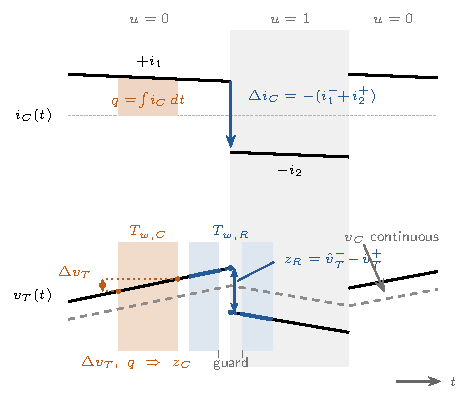
\includegraphics{fig02_observation_waveforms.pdf}
\caption{1.5个开关周期上的拓扑同步激励与解耦观测（示意图；保护带为可读性放大）。电容电流在$+i_1$与$-i_2$之间换流；内部电压$v_C$（虚线）连续，而端电压$v_T$携带ESR不连续量，由保护窗$T_{w,R}$内的局部拟合外推到共同边沿时刻重构。$T_{w,C}$上的电荷积分$q$与端点差$\Delta v_T$构成容值行。}
\label{fig:waveforms}
\end{figure}

\subsection{时间戳重构的ESR观测}

直接的边沿采样受采集偏斜、有限带宽与开关瞬态污染。因此，所提测量在边沿前后的安全窗口内对带时间戳的采样点拟合局部线性模型，并把两个模型外推到共同的开关时间戳，在同一物理时刻估计不连续量，而不是相减取自不同偏移时刻的样本。以重构截距$\hat v_T^-$与$\hat v_T^+$表示，被接受的ESR行为
\begin{equation}
z_R=\hat v_T^- -\hat v_T^+
=k_R I_\Sigma r_C+\nu_R,
\quad I_\Sigma=i_1^-+i_2^+,
\label{eq:esr_observation}
\end{equation}
其中$k_R$是训练锁定的标定系数，$\nu_R$汇集电压、时间戳、拟合与残余前端误差。

无诊断注入不意味着零传感负担。虽然第\ref{sec:modeling}节的测量集不新增传感器，但第\ref{sec:device}节的器件级实现对差分$v_T$模拟前端使用了绝对量程与边沿量程两档。不需要电容支路电流传感器。

仿真标定与盲健康辨识使用不相交的案例集。四个标定剖面——标称、高占空比/负载、高噪声、以及标称寄生Model~B——构成接受边沿比值
\begin{equation}
\kappa_m=\frac{z_{R,m}}{I_{\Sigma,m}r_{C,\mathrm{ref},m}},
\qquad
\hat k_R=\operatorname{median}_m\kappa_m,
\label{eq:kr_calibration}
\end{equation}
其中$r_{C,\mathrm{ref},m}$是植入的仿真参考ESR。所得训练锁定系数$k_R=0.9772$，按四位小数报告；全部再生结果所用的全精度值保留在补充说明S2与溯源记录中。

评估中，围绕$\hat k_R$声明的$\pm0.006$逐例散布代表标定后测量链增益的个体差异。对每个仿真案例，实现的系数在标定后视为已知，并通过$h_R=k_RI_\Sigma$完全相同地提供给所有对比估计器。因此该散布检验的是标定后的个体差异，而非残余未知标定误差；$k_R$绝不从盲残差中更新。硬件实现则需要在最终测量链下用独立表征的参考电容进行投运标定。

残余标定误差可解析刻画。若估计器被提供$\hat k_R=(1+\delta)k_R$而数据携带$k_R$，则无噪声极限下边沿行辨识出$r_C/(1+\delta)$：固定的相对标定误差$\delta$一一映射为$-\delta/(1+\delta)$的乘性ESR偏置。经式~\eqref{eq:c_mismatch}的补偿项，同一误差给容值行增加约$\delta\,r_C\Delta i_C$的贡献，相对电荷项的比值以$\delta\,|r_C\Delta i_C|\,C_b/(|q|\,\alphab)$为界。由于固定比例在$\hat r_C/\hat r_{C,0}$与$\hat C/\hat C_0$的比值中相消，健康趋势判断能够容忍恒定的残余标定误差，而绝对ESR仍需上述投运标定。

因此$k_R$在每个辨识区间内已知且固定；否则边沿行只能辨识乘积$k_Rr_C$。较小的评估包络值$k_{R,\min}^{\mathrm{eval}}=0.957654$仅用于保守信息下界，并不解除该尺度模糊性。

\subsection{安全窗电荷观测}

对完全处于单一开关状态内的区间$[t_a,t_b]$，记电荷安全窗长$T_{w,C}=t_b-t_a$，定义
\begin{equation}
q=\int_{t_a}^{t_b}i_C(t)\,dt.
\label{eq:charge}
\end{equation}
在该区间上对式~\eqref{eq:cap_port}积分，得
\begin{equation}
\Delta v_T=\frac{q}{C}+r_C\Delta i_C.
\label{eq:integral_port}
\end{equation}
使用最近一次被接受的ESR估计，得容值伪测量
\begin{equation}
z_C=\Delta v_T-\hat r_C\Delta i_C
=\frac{q}{C_b}\alphab+\nu_C.
\label{eq:c_observation}
\end{equation}
表~\ref{tab:observations}汇总了这两行。ESR估计不确定度与残余相关性进入条件测量协方差。

更明确地，对测得的端点电流、电压、电荷与前次ESR估计做一阶代入，得
\begin{multline}
z_C=\frac{q}{C_b}\alphab+(r_C-\hat r_C)\Delta i_C
+\nu_{\Delta v}-\hat r_C\nu_{\Delta i}+\nu_q,
\label{eq:c_mismatch}
\end{multline}
其中$\nu_q$是折算为电压的电荷积分误差。在所评估的实现中，其未缩放电荷方差记为$R_q$，即$\operatorname{var}(\nu_q)=\alphab^2R_q$。把前次ESR误差当作方差为$P_{rr}$的零均值条件不确定度处理，条件测量协方差可近似为
\begin{equation}
R_C\simeq R_{\Delta v}+(\Delta i_C)^2P_{rr}
+\hat r_C^2R_{\Delta i}+\alphab^2R_q.
\label{eq:c_covariance}
\end{equation}
这里$R_{\Delta v}=2R_v$，$R_{\Delta i}=2R_i$，$R_q$由电流噪声方差、ADC间隔与积分长度确定。式~\eqref{eq:c_covariance}传播的是不确定度；带偏差的$(r_C-\hat r_C)\Delta i_C$项仍是有界的模型失配，而非白噪声。

\begin{table}[t]
\caption{解耦观测行}
\label{tab:observations}
\centering
\begin{tabular}{p{0.9cm}p{2.35cm}p{2.3cm}p{1.5cm}}
\toprule
行 & 测量 & 回归 & 主导参数 \\
\midrule
边沿 & $\hat v_T^- -\hat v_T^+$ & $k_R I_\Sigma r_C+\nu_R$ & $r_C$ \\
电荷 & $\Delta v_T-\hat r_C\Delta i_C$ & $(q/C_b)\alphab+\nu_C$ & $\alphab$ \\
\bottomrule
\end{tabular}
\end{table}

\subsection{有效性与更新策略}

观测仅在CCM且时间戳、拓扑状态有效、安全窗完整时才被接受。以$\mathcal S_C$与$\mathcal S_R$记这些前置检查，共用评估流实现
\begin{equation}
\begin{aligned}
\mathcal V_C&=\mathrm{CCM}\wedge\mathcal S_C\wedge(n_C>0),\\
\mathcal V_R&=\mathrm{CCM}\wedge\mathcal S_R\wedge
(I_\Sigma\ge I_{\Sigma,\mathrm{gate}}),
\end{aligned}
\label{eq:gates}
\end{equation}
预声明$I_{\Sigma,\mathrm{gate}}=0.12$~A。电荷接受使用CCM/安全窗标志与非零接受电荷计数；实现中没有单独的数值$q_{\mathrm{gate}}$。归一化新息平方（NIS）阈值9可额外剔除\TSKF{}离群值。门控未通过时保持相应估计。第\ref{sec:identifiability}节的评估包络极小值是证明常数，不是在线阈值。

由于容值回归量$h_C=q/C_b$随接受电荷趋零，正信息保证只限于评估的有效CCM包络内，而不对任意小的$q$断言。


\section{有限窗可辨识性与信息下界}
\label{sec:identifiability}

\subsection{基于原始观测对的联合可辨识性}

可辨识性在原始观测上建立，先于任何顺序ESR补偿。把未补偿的电荷关系式~\eqref{eq:integral_port}写成$\Delta v_T=(q/C_b)\alphab+r_C\Delta i_C+\nu_{\Delta v}$，与边沿行~\eqref{eq:esr_observation}堆叠，得
\begin{equation}
\begin{bmatrix}\Delta v_T\\z_R\end{bmatrix}
=\vect{H}_k\,\vect{\theta}+\vect{\nu}_k,
\qquad
\vect{H}_k=
\begin{bmatrix}q/C_b&\Delta i_C\\0&k_RI_\Sigma\end{bmatrix}.
\label{eq:joint_obs}
\end{equation}
由于$\det\vect{H}_k=(q/C_b)\,k_RI_\Sigma$，只要$q\neq0$、$I_\Sigma\neq0$且$k_R\neq0$，$\vect{H}_k$即满秩。这些条件在所评估的有效CCM包络上成立：边沿电流条件由式~\eqref{eq:gates}显式强制，非零接受电荷由该包络内符号不变的CCM电荷窗保证，而$k_R\neq0$是固定的标定假设而非在线门控。对有限正定的原始观测协方差$\vect{R}_k$，联合Gram矩阵$\sum_k\vect{H}_k^{\mathsf T}\vect{R}_k^{-1}\vect{H}_k$对任何含至少一个完整接受观测对的窗口正定。在以被接受的重构回归量与固定标定系数为条件的意义下，$(\alphab,r_C)$由原始观测模型联合局部可辨识；由于$C=C_b/\alphab$在$\alphab>0$时局部一一对应，同样结论对$(C,r_C)$成立。该论断不涉及任何$r_C$的估计值。堆叠观测对仅是可辨识性构造：在线实现无需同时处理两行，后文的顺序下界也分别计数$m_C$个电荷行与$m_R$个边沿行。

\subsection{顺序实现的信息结构}

所实现的递推按式~\eqref{eq:joint_obs}的三角结构顺序处理：边沿行只含$r_C$，电荷行按式~\eqref{eq:c_observation}用最近的ESR估计补偿，其残差$(r_C-\hat r_C)\Delta i_C$经条件协方差式~\eqref{eq:c_covariance}传播而非被忽略。对该解耦流，回顾回归量$h_C=q/C_b$与$h_R=k_RI_\Sigma$及条件方差$R_C$与$R_R$；各方向的有限窗信息Gram矩阵为
\begin{equation}
\vect{G}_{\theta,N}=
\sum_{k\in\mathcal K_C}\frac{1}{R_{C,k}}
\begin{bmatrix}h_{C,k}^2&0\\0&0\end{bmatrix}
+
\sum_{k\in\mathcal K_R}\frac{1}{R_{R,k}}
\begin{bmatrix}0&0\\0&h_{R,k}^2\end{bmatrix}.
\label{eq:gramian}
\end{equation}

设在每个被接受的电荷区间上，电流满足$|i_C|\ge I_{C,\min}^{\mathrm{eval}}$且不改变符号，区间长度不小于$T_{w,C,\min}$，则$|q|\ge q_{\min}^{\mathrm{eval}}=I_{C,\min}^{\mathrm{eval}}T_{w,C,\min}$。若$R_C\le R_{C,\max}$且$R_R\le R_{R,\max}$，标定后的$k_R$保持固定并在评估包络上具有已知的保守下界$k_{R,\min}^{\mathrm{eval}}>0$，且$I_\Sigma\ge I_{\Sigma,\min}^{\mathrm{eval}}>0$，则包含$m_C$个电荷行与$m_R$个边沿行的窗口，其各方向信息下界为
\begin{align}
\underline\mu_C & =m_C\frac{(I_{C,\min}^{\mathrm{eval}}T_{w,C,\min}/C_b)^2}{R_{C,\max}},
\label{eq:mu_c}\\
\underline\mu_R & =m_R\frac{(k_{R,\min}^{\mathrm{eval}})^2(I_{\Sigma,\min}^{\mathrm{eval}})^2}{R_{R,\max}}.
\label{eq:mu_r}
\end{align}
由这些下界可得所实现流的如下结果。

\begin{proposition}[顺序实现的方向式有限窗信息正性]
\label{prop:identifiability}
假设：有效CCM；$k_R$在每个辨识窗内已知且固定；被接受电荷窗内符号不变；被接受边沿电流和为正；条件协方差有限；且有限窗内至少各有一个被接受的电荷行与边沿行。则
\begin{equation}
\vect{G}_{\theta,N}\succeq
\operatorname{diag}(\underline\mu_C,\underline\mu_R)\succ\vect{0},
\label{eq:positive_gramian}
\end{equation}
即所实现的顺序流在两个参数方向上都保持严格为正的有限窗信息。
\end{proposition}

\emph{证明：}每个电荷行仅在$\alphab$方向贡献一个半正定矩阵，每个边沿行仅在$r_C$方向贡献一个。应用式~\eqref{eq:mu_c}与~\eqref{eq:mu_r}中的物理下界，对$m_C$与$m_R$个被接受贡献求和，并注意两个下界均严格为正，即得式~\eqref{eq:positive_gramian}。\hfill$\square$

\begin{remark}[激励的条件性]
\label{rem:conditional}
仅靠PWM并不能在每个负载或导通模式下保证持续激励（PE）。\Cuk{}拓扑提供物理方向，而被接受的观测行证明该下界何时适用。上标"eval"表示在所评估CCM包络上取的极小值；这些常数既不是在线门限，也不是事后调参值。
\end{remark}

\subsection{数值下界校验}

命题~\ref{prop:identifiability}的常数在评估包络上实例化如下。在45个独立的Model~B CCM案例上，最弱的物理量为
\begin{align}
I_{C,\min}^{\mathrm{eval}}&=0.330108~\mathrm{A},&
I_{\Sigma,\min}^{\mathrm{eval}}&=0.438504~\mathrm{A},\nonumber\\
q_{\min}^{\mathrm{eval}}&=0.660217~\mu\mathrm{C}&&
\end{align}
其中$T_{w,C,\min}=2.0~\mu$s，$k_{R,\min}^{\mathrm{eval}}=0.957654$。由此得到的最弱信息下界为
\begin{equation}
\underline\mu_C=0.217943,\qquad
\underline\mu_R=880.008.
\label{eq:numerical_mu}
\end{equation}
经验信息与相应保守下界之比的最小值分别为1.02872与1.02334。因此每个保留案例都超过其计算下界，且报告常数由最弱案例而非标称案例决定；图~\ref{fig:pe_lower_bound}给出全部保留案例的经验信息与相应下界的对比。这些存在性下界由第\ref{sec:results}节的条件CRLB基准补充，后者量化实际估计器方差与被接受行信息的接近程度。

\begin{figure}[t]
\centering
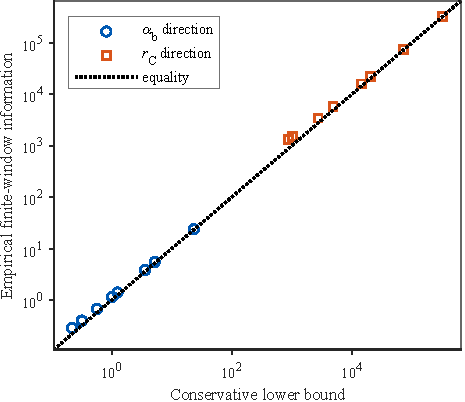
\includegraphics{fig_pe_lower_bound.pdf}
\caption{Model~B CCM案例上的理论下界与经验有限窗信息对比。圆圈为归一化逆电容方向，方块为物理ESR方向；二者量纲与量级依赖参数化方式，不可直接比较。全部被接受案例位于等值线上方。}
\label{fig:pe_lower_bound}
\end{figure}

\subsection{面向不确定度扩展的协方差收缩}

对于第\ref{sec:estimators}节的区间报告扩展，设$P_n$为后验方差，$Q_N$为有限窗内累积的过程方差，$\mu\ge\underline\mu>0$为被接受的信息。

\begin{proposition}[有限窗协方差有界性]
\label{prop:covariance}
对反复出现的有效更新、有限的$0\le Q_N\le\bar Q_N$以及$\mu\ge\underline\mu>0$，后验方差满足
\begin{equation}
P_{n+1}\le
\frac{P_n+Q_N}{1+\mu(P_n+Q_N)}.
\label{eq:cov_recursion}
\end{equation}
对常数$Q_N$，式~\eqref{eq:cov_recursion}的正不动点为
\begin{equation}
P^*=\frac{-Q_N+\sqrt{Q_N^2+4Q_N/\mu}}{2}.
\label{eq:fixed_point}
\end{equation}
当$Q_N=0$时，$P_n^{-1}\ge P_0^{-1}+n\mu$。
\end{proposition}

\emph{证明：}见附录~\ref{app:covariance}，其中同时给出经验证的不动点数值。\hfill$\square$

\begin{remark}[收缩结果的适用范围]
\label{rem:contraction_scope}
命题~\ref{prop:covariance}是与标准滤波理论\cite{jazwinski1970filtering,anderson1979optimal}一致的条件性线性模型结果，不是全局非线性变换器收敛定理。在200个合法PE种子中投影从未激活，故投影被视为安全约束而非收缩的来源。
\end{remark}

\section{在线估计：估计核与监督重置实现}
\label{sec:estimators}

本节的所有实现消费第\ref{sec:observations}节的同一组被接受边沿行与电荷行，从而把观测效应与递推核效应分离。首先给出两个估计核基线，随后剥离其跟踪--置信权衡，最后给出监督重置实现。

\subsection{估计核基线}
\label{sec:kernels}

轻量基线\TSRLS{}——拓扑同步方向解耦RLS——对每个健康方向使用一个标量RLS递推。对方向$j\in\{C,R\}$，一条被接受的行$z_{j,k}=h_{j,k}\theta_{j,k}+\nu_{j,k}$触发更新
\begin{align}
K_{j,k}&=\frac{P_{j,k-1}h_{j,k}}
{\lambda+h_{j,k}^{2}P_{j,k-1}},
\label{eq:rls_gain}\\
\hat\theta_{j,k}&=\hat\theta_{j,k-1}
+K_{j,k}(z_{j,k}-h_{j,k}\hat\theta_{j,k-1}),
\label{eq:rls_state}\\
P_{j,k}&=\lambda^{-1}(P_{j,k-1}-K_{j,k}h_{j,k}P_{j,k-1}),
\label{eq:rls_cov}
\end{align}
其中预声明遗忘因子$\lambda=0.9975$；$\lambda$越大估计越平滑，代价是整定时间越长。只有与被接受观测相关联的方向才被更新，有效性门控剔除不满足预声明接受规则的行，投影把参数约束在物理区间内。报告的健康量为$\hat C=C_b/\hat\alphab$与$\widehat{\ESR}=\hat r_C$。

Kalman核\TSKF{}——拓扑同步标量线性时变（LTV）Kalman估计器——维护结构化状态$\vect{x}_k=[v_{C,k}\;\alphab_k\;r_{C,k}]^{\mathsf T}$，其电荷驱动转移为
\begin{equation}
\vect{F}_k=
\begin{bmatrix}
1&q_k/C_b&0\\0&1&0\\0&0&1
\end{bmatrix}.
\label{eq:kf_transition}
\end{equation}
结构化测量方向$\vect{H}_V=[1,0,0]$、$\vect{H}_C=[0,q/C_b,0]$与$\vect{H}_R=[0,0,k_RI_\Sigma]$进入标量Joseph形式协方差更新，过程与测量协方差均预声明；NIS门控使用预声明门限$\gamma=9$。后验协方差提供有校准的区间报告。两个核都是标准递推\cite{jazwinski1970filtering,anderson1979optimal}；均不声称新颖性，TS-前缀仅表示其拓扑同步、方向专属的使用方式。

\subsection{无监督核的跟踪--置信权衡}
\label{sec:tradeoff}

两个核以互补的方式失效。RLS基线跟踪与恢复迅速，但其辅助的残差加权区间未经校准（第\ref{sec:results}节中联合覆盖率$13.00\%$）。Kalman核报告接近名义值的同时覆盖率（$88.93\%$），但健康参数突变后每个新息都超过NIS门，更新被拒绝，协方差保持很小，估计冻结在陈旧值——这是无监督实现被保留的负结果。该机理同时指出了缺失的信息：被门拒绝的新息虽被点更新丢弃，却携带着参数变化的持续同号证据。

\subsection{主实现：监督重置估计器\TSSRKE{}}
\label{sec:srke}

\begin{figure*}[!t]
\centering
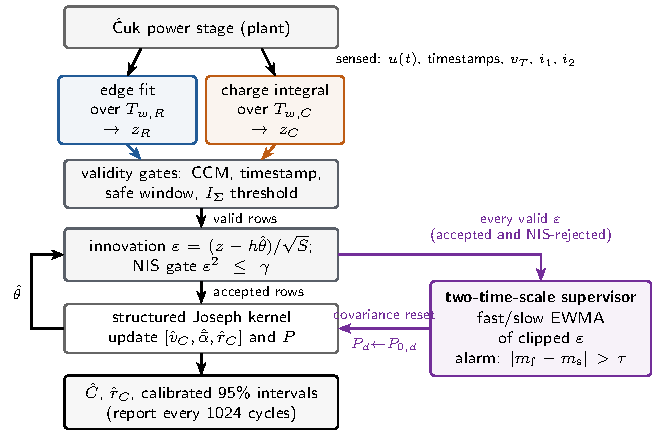
\includegraphics{fig03_estimation_loop.pdf}
\caption{完整的监督估计回路：由感测波形逐周期提取特征构成两行观测；式~\eqref{eq:gates}的有效性门控放行有效行；新息$\varepsilon$由反馈估计$\hat\theta$构建并经NIS门筛选，被接受的行更新结构化Joseph核。双时间尺度监督器监视\emph{每一个}有效$\varepsilon$——无论被接受还是被NIS拒绝——在持续偏移后通过方向专属协方差重置恢复增益；未通过有效性门控的行不产生新息并保持估计。}
\label{fig:loop}
\end{figure*}

\TSSRKE{}在Kalman核上叠加方向专属监督器，闭合图~\ref{fig:loop}所示的回路。监督器监视\emph{每一个}有效行（无论被接受还是被拒绝）的削波归一化新息
\begin{equation}
\varepsilon_{j,k}=\operatorname{clip}\!\left(\frac{z_{j,k}-h_{j,k}\hat\theta_{j,k-1}}{\sqrt{S_{j,k}}},\pm c\right),
\quad S_{j,k}=h_{j,k}^2P_{j}+R_{j,k}.
\label{eq:eps}
\end{equation}
两个时间尺度分离的指数加权均值（EWMA）
\begin{equation}
\begin{aligned}
m^{\mathrm f}_{j}&\leftarrow m^{\mathrm f}_{j}+a_{\mathrm f}\,(\varepsilon_{j,k}-m^{\mathrm f}_{j}),\\
m^{\mathrm s}_{j}&\leftarrow m^{\mathrm s}_{j}+a_{\mathrm s}\,(\varepsilon_{j,k}-m^{\mathrm s}_{j}),
\end{aligned}
\label{eq:twoscale}
\end{equation}
分别充当当前新息水平与其偏置基准。当$|m^{\mathrm f}_{j}-m^{\mathrm s}_{j}|>\tau$时，监督器把该方向的协方差重置为初始化值，重锚$m^{\mathrm f}_{j}\leftarrow m^{\mathrm s}_{j}$，并在随后$N_{\mathrm h}$个有效行内暂禁；解禁武装需要每方向$N_{\mathrm w}$行的学习窗。全部常数预声明且两方向共享：$a_{\mathrm f}=1/16$与$a_{\mathrm s}=1/128$（八倍时间尺度分离）、$\tau=2.5$、$c=6$、$N_{\mathrm w}=N_{\mathrm h}=32$。

双时间尺度形式是刻意选择。残余时间偏斜在边沿行中留下确定性的近周期扰动，其$\sigma$归一化幅值随噪声减小而增大；朴素CUSUM会在其上误报警，而快滤波器把这一零均值扰动衰减到$\tau$以下，持续的参数变化偏移则在几个有效行内越过$\tau$。重置后Kalman增益恢复，估计如同从初始化重新收敛，报告区间先展宽再收紧，与变化后增大的不确定度相一致。监督器在核之上对每个有效行仅增加4次乘法与约7次加法/比较。其组件——EWMA残差滤波、变化监督、协方差重置——都是经典的\cite{page1954cusum,mehra1970adaptive,willsky1976survey,gustafsson2000adaptive}；贡献在于它们在门控拓扑同步观测行上的方向专属构造。

\section{验证方法学}
\label{sec:protocol}

本节声明第\ref{sec:results}节与第\ref{sec:device}节全部结果所消费的模型、对比、公平规则与指标；每个阈值与超参数都在盲评估之前固定，此后绝不重调。全部模型与估计器在MATLAB（R2023b）中实现。

\subsection{模型与数据层级}

评估把方程校核、独立对象轨迹、估计器对比与器件级采集分离开：
\begin{enumerate}
\item Model~A是开关方程\Cuk{}模型，用于符号、时序与快速动态校核。
\item Model~B是独立构建的Simscape模型；其45条轨迹标定电流尺度与边沿斜率，并提供盲观测数据。
\item 估计器对比使用48个分层盲工况/健康案例、四档噪声与四档残余时间偏斜，共享同一O1观测。
\item F28379D模型加入寄存器可实现的采样、孔径/占用、基准/时钟效应、模拟前端（AFE）残差与Monte Carlo变差；它仍是仿真。
\end{enumerate}
补充的闭环调节与轻载可用性研究在Model~A周期上复用锁定管线，条件CRLB研究把估计器误差与纯噪声下界作基准对比；三者均在第\ref{sec:results}节报告。

\subsection{因子分解与盲对比}

观测--估计器因子分解把通用混合观测基线（O0）与所提方向解耦观测集（O1）与四个估计器交叉：RLS（E1）、双扩展Kalman滤波器（Dual EKF，E2）、结构化LTV/Joseph估计器（E3）与监督重置估计器（E4，\TSSRKE{}）。O0有明确定义：每次更新使用单一非解耦行$\Delta v_T=(q/C_b)\alphab+\Delta i_C\,r_C+\nu$，由通用周期内采样构成，保留原始采集滞后贡献且不做边沿时间戳重构，容值与ESR因此共享一个耦合回归。O0并不声称复现任何单一已发表方法；它代表丢弃拓扑同步边沿重构的通用耦合周期内观测。O1把该行换成第\ref{sec:observations}节的解耦观测对。两个观测集使用相同传感器、相同种子、每个估计器族一套预声明超参数，因此因子分解隔离的正是观测结构本身。全部$2\times4\times768=6144$条配对行均被保留；由于观测流按条件播种并共享，E1--E3行与监督器加入前的原campaign逐位一致。最终对比在O1下把\TSSRKE{}与\TSRLS{}、\TSKF{}、Dual EKF比较，主方法遴选判据预先声明：稳态行为与Kalman母体偏差在$2\%$以内、突变整定不劣于两个保留实现（\TSRLS{}与\TSKF{}）、覆盖率与母体相差两个百分点以内、负载瞬态虚假健康峰值不更差。

更广的基线研究包含闭式解、混合RLS、增广/Dual-EKF与\Cuk{}适配的小波--Kalman方法。一种NPC频谱方法被排除，因为文献没有给出到\Cuk{}边沿/电荷约定的唯一映射。

\subsection{公平规则与指标}

所有方法使用完全相同的盲案例、观测、种子、初始化分布、噪声/时序实现与预声明超参数；表~\ref{tab:verification_settings}列出盲验证与估计器设置。失败或饱和的行照常保留，盲评估后不对任何方法重调，配对效应使用10\,000次bootstrap重采样。重采样把案例--条件行视为可交换单元并保持估计器配对；共享同一基础对象案例的行并不独立，因此所报告区间量化的是所评估网格上的不确定度，而非独立变换器总体上的不确定度。

突变的C/ESR不连续是估计器压力测试。主要动态案例是持续$0.1$、1、10、100~s的线性与平滑C下降、ESR上升及联合斜坡。长斜坡使用轨迹推导的O1充分统计量，$0.1$~s案例则与Model~A逐开关对交叉校核。负载、输入电压与占空比切换保持健康不变，用于测量虚假健康响应。这些轨迹均非硬件老化数据。

\begin{table*}[t]
\caption{盲验证与估计器设置}
\label{tab:verification_settings}
\centering
\setlength{\tabcolsep}{4pt}
\small
\begin{tabular}{p{2.6cm}p{6.2cm}p{6.2cm}}
\toprule
项目 & 预声明设置 & 角色/来源边界 \\
\midrule
健康/负载矩阵 & $C/C_b\in\{0.8,0.9,1.0\}$；$r_C/r_b\in\{1,1.5,2\}$；负载系数$0.58/1/1.45$ & 分层盲对象矩阵；仅保留CCM行 \\
初始化 & 实现值$\hat C_0/C\in[0.708,1.287]$；$\hat r_{C,0}/r_C\in[0.512,1.483]$ & 从盲例表读取 \\
参数界 & $C/C_b\in[0.65,1.35]$；$r_C/r_b\in[0.35,2.50]$ & 预声明投影界；失败/饱和行保留 \\
噪声档 & $(\sigma_v,\sigma_i)=(1~\mathrm{mV},0.5~\mathrm{mA})$、$(5~\mathrm{mV},2~\mathrm{mA})$、$(10~\mathrm{mV},5~\mathrm{mA})$、$(2.2~\mathrm{mV},1.2~\mathrm{mA})$ & 共享实现；最后一档为F28379D现实档 \\
残余偏斜 & 0、20、50、100~ns & 全部对比估计器共享 \\
在线有效性/门控 & 有效CCM/状态/时间与安全特征；$I_{\Sigma,\mathrm{gate}}=0.12$~A；无数值$q_{\mathrm{gate}}$；\TSKF{} NIS门9 & 评估前固定，非由PE极小值推得 \\
评估PE常数 & $I_{C,\min}^{\mathrm{eval}}=0.330108$~A；$I_{\Sigma,\min}^{\mathrm{eval}}=0.438504$~A；$q_{\min}^{\mathrm{eval}}=0.660217~\mu$C & 45个评估Model-B CCM案例上的极小值；仅用于证明，绝非在线整定阈值 \\
盲对比 & 48案例$\times$4噪声$\times$4偏斜；O0/O1 $\times$ RLS/Dual EKF/LTV-Joseph/\TSSRKE{} & 随后O1为四个估计器共享 \\
统计/动态 & 10\,000次配对bootstrap重采样；$0.1/1/10/100$~s的C、ESR与联合斜坡 & 负载、输入电压与占空比阶跃保持物理健康不变 \\
\TSKF{}设置 & $Q_\alpha=2\times10^{-9}$、$Q_r=5\times10^{-9}$、$P_{0,\alpha}=0.0144$、$P_{0,r}$尺度0.45、NIS 9 & 盲对比前固定；\TSSRKE{}核共享 \\
\TSSRKE{}监督器 & $a_{\mathrm f}=1/16$、$a_{\mathrm s}=1/128$、$\tau=2.5$、削波6、预热/暂禁各32行 & 预声明，两方向共享；绝不逐例重调 \\
器件采集 & 每模块1.093~MS/s；$0.5~\mu$s保护带；$T_{w,R}=2.2~\mu$s；每侧三点 & 仅限受约束的F28379D仿真 \\
\bottomrule
\end{tabular}
\end{table*}

静态端点误差为
\begin{equation}
e_C=100\left|\hat C_N/C-1\right|,\quad
e_R=100\left|\hat r_{C,N}/r_C-1\right|,
\end{equation}
在保留行上计算平均绝对百分比误差（MAPE）与95百分位（p95）。区间校准以联合覆盖率报告——即容值与ESR的边缘95\%区间同时覆盖各自真值的保留行比例；在近似独立下其名义基准为$0.95^2\approx90.25\%$。“收敛周期数”是首个开启连续32周期、两个相对误差均在$5\%$以内的周期；未收敛案例记为1024周期上限。被拒绝的周期保持估计并计入周期数。该内部整定指标不同于1024周期（$20.48$~ms）的对外报告节拍。

对轨迹$y(t)$与初始真值$y_0$，所实现的跟踪指标为
\begin{equation}
\operatorname{nRMSE}_y=
\sqrt{\frac{\int(\hat y-y)^2dt}{\int(y-y_0)^2dt}}.
\end{equation}
联合nRMSE是有限的C与ESR值的无权平均。归一化滞后是由零均值互相关与$50\%$轨迹穿越两种方式估计的最大有限C/ESR延迟除以轨迹时长。错过的阈值穿越照常保留，但不用于主估计器遴选。补充说明S3记录完整的阈值与bootstrap定义。

\section{结果}
\label{sec:results}

\subsection{观测框架的归因}

观测--估计器因子分解提供最清晰的归因。在保持E1 RLS核不变的情况下把O0换成O1，平均容值MAPE从$7.0366\%$降到$0.3727\%$，平均ESR MAPE从$1.1970\%$降到$0.2233\%$，平均内部收敛从$665.41$降到$13.21$个开关周期。配对ESR降幅为$0.97369$个百分点（95\% bootstrap区间0.92352--1.0265）；全部4608行均保留。其余配对区间见补充说明S3。

O1还使Dual EKF与E3 LTV/Joseph的容值MAPE下降超过6.7个百分点；图~\ref{fig:observation_effect}给出带bootstrap区间的配对效应。改进并非普适：Dual-EKF的ESR-p95效应为负，其区间不支持O1。因此，因子分解支持观测框架，但不意味着每个估计器指标都单调改善。

\begin{figure}[t]
\centering
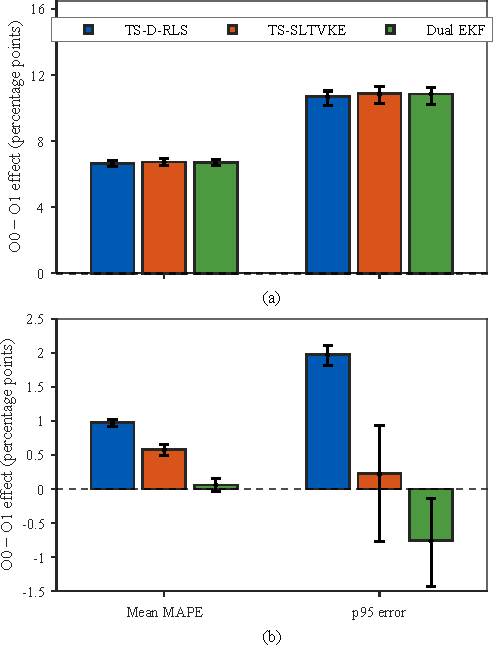
\includegraphics{fig_observation_effect.pdf}
\caption{配对O0--O1对MAPE与p95误差的效应（带bootstrap区间）：(a)~容值；(b)~ESR。正值有利于拓扑解耦的O1观测；不利的Dual-EKF ESR-p95效应照常保留。}
\label{fig:observation_effect}
\end{figure}

\subsection{O1下的静态估计器对比}

表~\ref{tab:static_estimators}在$48\times4\times4$的O1矩阵上比较四个候选，图~\ref{fig:static_comparison}可视化平均误差；无一发散。受监督的\TSSRKE{}在每个静态指标上都\emph{逐位}复现其Kalman母体——监督器在全部768个盲行上保持沉默，包括承载最大确定性边沿扰动的低噪声/高偏斜格。\TSRLS{}保持最低ESR误差与最快原生收敛，这一基线优势全程如实报告。按第\ref{sec:protocol}节的预声明遴选判据，计入下述动态结果后\TSSRKE{}被采纳为主实现；\TSRLS{}保留为轻量跟踪备选。

\begin{table}[t]
\caption{静态O1估计器对比（含内部收敛）}
\label{tab:static_estimators}
\centering
\setlength{\tabcolsep}{4pt}
\begin{tabular}{lrrrr}
\toprule
方法 & C MAPE & ESR MAPE & C/ESR p95 & 收敛 \\
 & (\%) & (\%) & (\%) & (内部周期) \\
\midrule
\TSRLS{} & 0.3727 & \textbf{0.2233} & 1.3182/0.7002 & \textbf{13.21} \\
\TSKF{} & \textbf{0.3011} & 0.6446 & 1.1069/2.4992 & 33.09 \\
Dual EKF & 0.3043 & 1.1938 & 1.1492/3.8602 & 40.58 \\
\TSSRKE{} & \textbf{0.3011} & 0.6446 & 1.1069/2.4992 & 33.09 \\
\bottomrule
\end{tabular}
\vspace{1mm}

\begin{minipage}{\columnwidth}
\footnotesize \TSSRKE{}行与其Kalman母体逐位相等：监督器在全部768个静态盲行上保持沉默。
\end{minipage}
\end{table}

\begin{figure}[t]
\centering
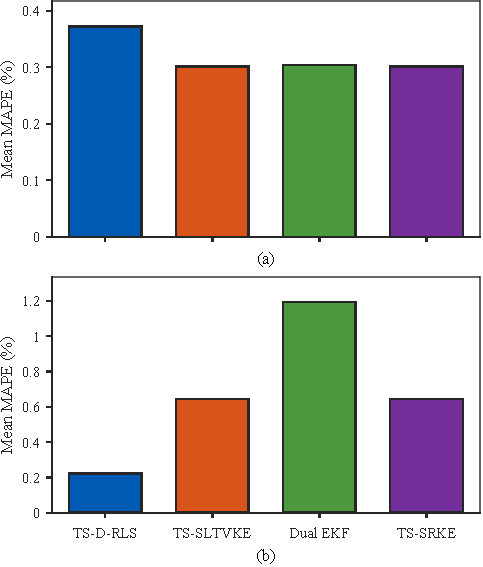
\includegraphics{fig_static_comparison.pdf}
\caption{共享O1观测下的静态平均MAPE：(a)~容值；(b)~ESR。\TSSRKE{}柱与\TSKF{}柱重合，因为监督器在稳态保持沉默。}
\label{fig:static_comparison}
\end{figure}

\subsection{噪声与时序鲁棒性}

四档噪声与0、20、50、100~ns残余时间偏斜的全部组合均保留。在F28379D现实噪声、50~ns偏斜下，C/ESR p95误差分别为\TSRLS{}的$0.4964\%/0.3385\%$、\TSKF{}的$0.4132\%/0.6888\%$与Dual EKF的$0.4211\%/1.9141\%$；\TSSRKE{}行在每个噪声/偏斜格都与\TSKF{}重合。图~\ref{fig:noise_timing}可视化该器件现实档；C与ESR百分位分开展示，因为二者的算术平均没有独立含义。

\begin{figure}[t]
\centering
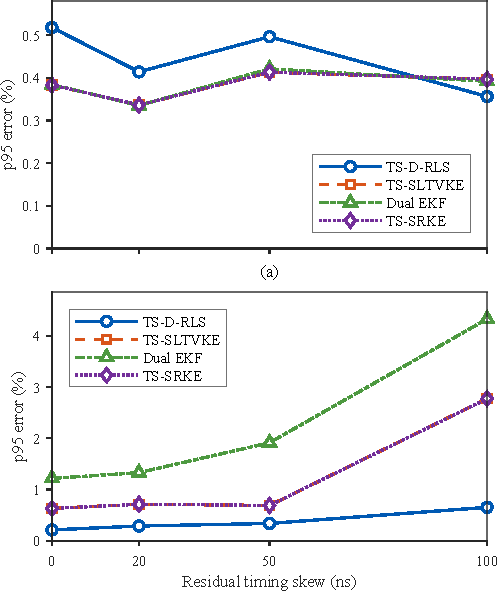
\includegraphics{fig_noise_timing.pdf}
\caption{F28379D现实噪声档、共享O1观测下p95误差随残余时间偏斜的变化：(a)~容值；(b)~ESR。\TSSRKE{}曲线与其Kalman母体完全重合；线型与标记的差异保证灰度下方法可辨。}
\label{fig:noise_timing}
\end{figure}

\subsection{条件CRLB基准}

条件CRLB由结构化估计器谱系（第\ref{sec:estimators}节）的被接受行信息计算，基于Model-A轨迹经寄存器标称测量链，覆盖负载、占空比、ADC速率、AFE带宽与时序共十五个敏感性案例、每案例二十个种子。当测量链与投运配置一致时，经验RMSE保持在下界的1.38--2.34倍（容值）与1.35--3.27倍（ESR）以内；十五案例的中位数为2.17与2.40（图~\ref{fig:crlb}）。偏离投运配置的情形则表现为噪声下界不建模的偏置：AFE带宽降至1.5~MHz使容值比升到25.0，带宽升至3~MHz使ESR比升到10.2，100/200~ns残余时间偏斜使容值比升到13.0/39.6。因此该下界充当条件信息基准：在投运配置处噪声驱动误差保持在其小倍数以内，偏离该配置的情形则标记标定或时序偏置。

\begin{figure}[t]
\centering
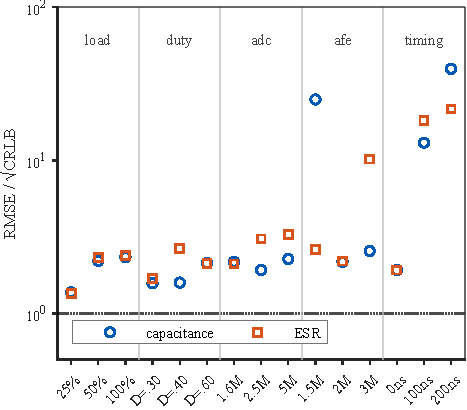
\includegraphics{fig_crlb_efficiency.pdf}
\caption{十五个敏感性案例（各二十种子）上经验RMSE相对条件CRLB的比值，按维度分组。该下界以被接受行为条件且只建模噪声，故远大于1的比值指示标定或时序偏置，而非估计器低效。}
\label{fig:crlb}
\end{figure}

\subsection{突变恢复：解决被保留的失效}
\label{sec:abrupt}

突变不连续是恢复压力测试，不是老化事件。在冻结的阶跃后257周期检查点（$\approx5.1$~ms）处，无监督的\TSKF{}仍带有$19.2911\%$（$C\rightarrow0.8C$后）与$49.9384\%$（$r_C\rightarrow2r_C$后）的误差：参数一旦跳变，每个新息都超过NIS门，估计随即冻结。在完整时程上（表~\ref{tab:abrupt}；整定时间自健康变化时刻起、按原生逐周期节拍测量），其容值阶跃迟至$64.72$~ms才整定，ESR与联合阶跃则始终不恢复。\TSSRKE{}在$1.52$、$0.48$与$1.20$~ms内整定容值、ESR与联合阶跃——远小于一个$20.48$~ms对外报告间隔——而\TSRLS{}需$10.72$--$17.68$~ms。在对外报告节拍下，恢复在第一或第二个报告样本处可见，取决于阶跃与报告的对齐（图~\ref{fig:abrupt}）。Dual EKF因不带门控而以最快速度（$0.24$~ms）整定ESR阶跃，但其未校准覆盖率、最差虚假ESR瞬态与最高成本不变，故仍被第\ref{sec:protocol}节的预声明遴选判据排除。

\begin{table}[t]
\caption{冻结压力流上的突变阶跃整定（自健康变化时刻起，原生逐周期节拍）}
\label{tab:abrupt}
\centering
\setlength{\tabcolsep}{4pt}
\begin{tabular}{lrrr}
\toprule
方法 & $C\!\rightarrow\!0.8C$ & $r_C\!\rightarrow\!2r_C$ & 联合 \\
 & (ms) & (ms) & (ms) \\
\midrule
\TSRLS{} & 10.72 & 17.68 & 17.28 \\
\TSKF{} & 64.72 & 不恢复 & 不恢复 \\
Dual EKF & 61.00 & \textbf{0.24} & 61.36 \\
\TSSRKE{} & \textbf{1.52} & 0.48 & \textbf{1.20} \\
\bottomrule
\end{tabular}
\end{table}

\begin{figure}[t]
\centering
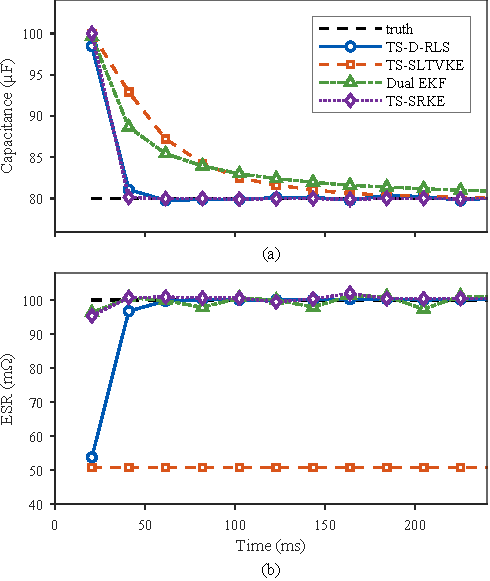
\includegraphics{fig_abrupt_recovery.pdf}
\caption{相同冻结流上突变健康阶跃后按报告节拍的恢复：(a)~$C\rightarrow0.8C$后的容值估计；(b)~$r_C\rightarrow2r_C$后的ESR估计。无监督\TSKF{}冻结在陈旧值；\TSSRKE{}在第一或第二个报告样本处重回误差带，取决于阶跃与报告的对齐。}
\label{fig:abrupt}
\end{figure}

\subsection{慢退化跟踪}

在表~\ref{tab:ramps}的$0.1$--$100$~s扫掠中，\TSRLS{}在全部四个时长上具有更低的联合nRMSE与归一化滞后汇总值，受监督的\TSSRKE{}则在舍入精度内跟随其Kalman母体：慢漂移保持在监督器阈值之下，因此解决突变阶跃的重置在健康现实的斜坡上刻意不触发（孤立触发使10~s汇总值略有改善）。轻量基线因此保有真实的斜坡跟踪优势，如实报告；图~\ref{fig:joint_ramp}给出对照植入真值的代表性联合轨迹。个别轨迹仍可能偏向Kalman侧；一个10~s C斜坡案例即如此。

\begin{table}[t]
\caption{慢退化跟踪汇总（M1=\TSRLS{}，M2=\TSKF{}，M4=\TSSRKE{}）}
\label{tab:ramps}
\centering
\setlength{\tabcolsep}{4pt}
\begin{tabular}{rrrrrrr}
\toprule
斜坡 & \multicolumn{3}{c}{联合nRMSE} & \multicolumn{3}{c}{归一化滞后 (\%)}\\
\cmidrule(lr){2-4}\cmidrule(lr){5-7}
(s) & M1 & M2 & M4 & M1 & M2 & M4 \\
\midrule
0.1 & 0.1161 & 0.2160 & 0.2160 & 8.053 & 22.027 & 22.027 \\
1   & 0.0163 & 0.0454 & 0.0454 & 1.360 & 3.537 & 3.537 \\
10  & 0.0160 & 0.0456 & 0.0449 & 1.752 & 4.492 & 4.492 \\
100 & 0.0213 & 0.0477 & 0.0478 & 2.827 & 4.868 & 4.868 \\
\bottomrule
\end{tabular}
\end{table}

\begin{figure*}[t]
\centering
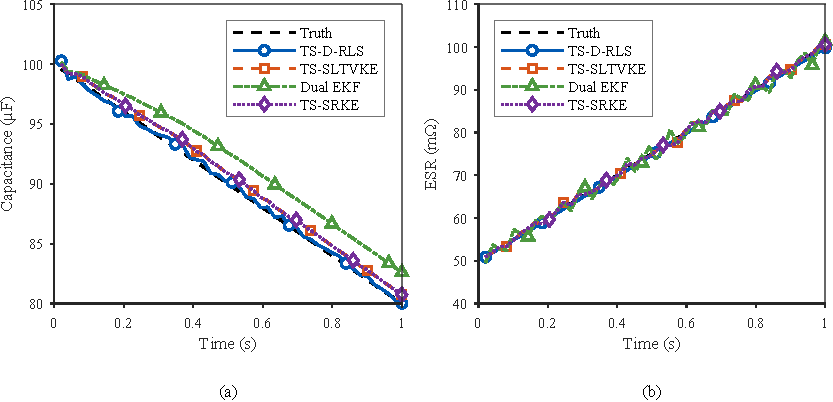
\includegraphics{fig_joint_ramp.pdf}
\caption{代表性联合健康斜坡：(a)~容值下降与(b)~ESR上升轨迹及植入真值。长时程轨迹使用轨迹推导的O1充分统计量，而非完整Simscape瞬态或实测老化数据。}
\label{fig:joint_ramp}
\end{figure*}

\subsection{工作点瞬态免疫}

负载、输入电压与占空比切换保持健康不变。\TSKF{}降低平均虚假C峰值（$0.7570\%$对$1.3017\%$），而\TSRLS{}降低平均虚假ESR峰值（$1.8474\%$对$5.1919\%$）且恢复更快。受监督的\TSSRKE{}在每个瞬态行上复现其母体——工作瞬态不触发任何重置，监督器自身不增加虚假健康响应。两个核家族都不全面主导工作瞬态免疫；补充图S4给出保留的负载阶跃轨迹。

\subsection{闭环运行}

此前所有行均保持占空比指令开环。补充研究围绕Model-A对象闭合一个刻意简化的低带宽离散PI电压环（占空比量化$0.5\%$），并在反馈下重新投运边沿增益（$k_R^{\mathrm{cl}}=0.9987$）；该研究与下面的轻载研究均以轻量\TSRLS{}实现评估观测管线。三个盲健康案例随后在30~ms处施加$1.45\times$负载阶跃、$+20\%$输入电压阶跃与16至12~V基准阶跃。稳态尾部容值与ESR误差保持在$0.222\%$与$0.111\%$以下，内部收敛需3--7周期，最大切换后偏移为容值$0.410\%$与ESR $0.102\%$（图~\ref{fig:closedloop}）。输入电压瞬态期间$15.7\%$的周期未通过CCM门而被拒绝并保持估计；精度不受影响。该研究每案例使用一个噪声种子，且不评估控制器设计本身。

第二个补充在同一调节器下运行受监督实现本身，复用冻结的闭环边沿增益与监督器常数。在额定、$1.45\times$负载阶跃与16至12~V基准阶跃案例中，监督器从不触发，虚假健康峰保持在$0.50\%$以下——调节器瞬态不会伪装成健康变化。在反馈下，$r_C\rightarrow2r_C$突变使监督器在阶跃后10个周期触发一次并以$0.20$~ms整定；$C\rightarrow0.8C$突变触发一次并以$0.28$~ms整定（图~\ref{fig:srke_closedloop}）。无监督母体在1500周期（30~ms）阶跃后时程内两种阶跃均不恢复：ESR阶跃后冻结于$49.95\%$的ESR误差——并经补偿项诱发$7.69\%$的容值误差——C阶跃后冻结于$19.70\%$的容值误差。受监督运行的尾部误差保持在$0.26\%$以下；每案例使用一个噪声种子。

\begin{figure}[t]
\centering
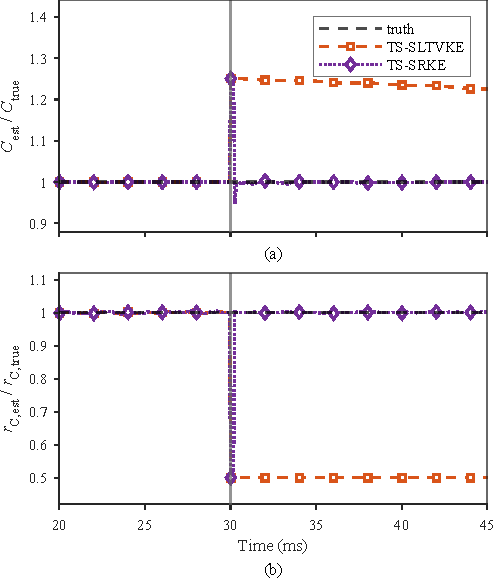
\includegraphics{fig_srke_closedloop.pdf}
\caption{闭环调节下、相同噪声流上的监督恢复，估计按时变真值归一化：(a)~$C\rightarrow0.8C$阶跃；(b)~$r_C\rightarrow2r_C$阶跃，均在30~ms处（灰线）。无监督母体冻结在阶跃前值；\TSSRKE{}触发一次并在$0.28$~ms内回到单位线。}
\label{fig:srke_closedloop}
\end{figure}

\begin{figure}[t]
\centering
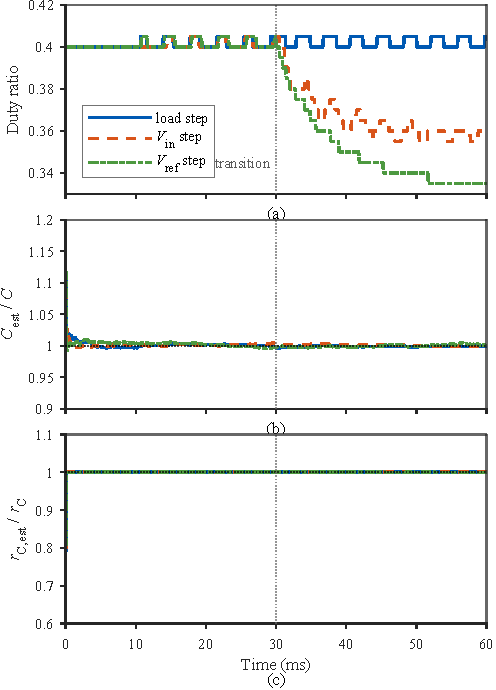
\includegraphics{fig_closedloop.pdf}
\caption{闭环补充研究：(a)~调节器占空比对30~ms处负载、输入电压与基准切换的响应；(b)、(c)~归一化容值与ESR估计。输入电压瞬态期间未通过CCM门的周期被拒绝并保持估计。}
\label{fig:closedloop}
\end{figure}

\subsection{轻载边界处的可用性}

由于可辨识性以有效CCM为条件，固定占空比扫掠用同一锁定管线量化从$100\%$到$6.7\%$负载的观测可用性。稳态周期接受率降至$20\%$负载前保持$100\%$，在$16.7\%$、$14.3\%$、$12.5\%$与$10.0\%$负载处降为$68.8\%$、$49.8\%$、$36.1\%$与$9.9\%$，在$8.3\%$负载及以下降为零，此时估计保持（图~\ref{fig:lightload}）。在完全可用范围内内部收敛从5周期延长到39周期，被接受行上的端点误差在$10\%$负载以上保持$1.4\%$以下。开关方程Model-A标记潜在DCM周期但不仿真DCM导通\cite{madrid2021dcm}；因此该扫掠量化的是可用性，而非DCM模式精度。

\begin{figure}[t]
\centering
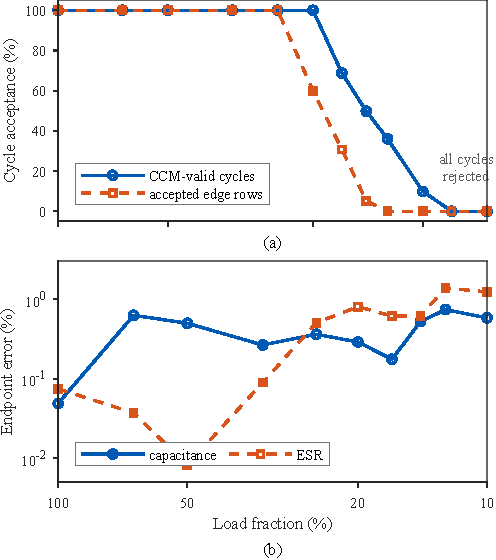
\includegraphics{fig_lightload.pdf}
\caption{固定占空比下的轻载可用性扫掠：(a)~稳态CCM有效周期与接受边沿行比例；(b)~被接受周期上的端点误差。低于可用性拐点后门控拒绝全部周期并保持估计。}
\label{fig:lightload}
\end{figure}

\subsection{复杂度与不确定度}

在表~\ref{tab:complexity}的共同算术基准上，\TSRLS{}、\TSKF{}、Dual EKF与\TSSRKE{}每个被接受观测分别需要28、46、62与50次乘法；监督器在其核之上花费4次乘法与约7次加法/比较。对照第\ref{sec:protocol}节$\approx90.25\%$的独立性基准，四者的联合区间覆盖率分别为$13.00\%$、$88.93\%$、$81.90\%$与$88.93\%$。因此\TSSRKE{}以每行4次额外乘法换取其母体接近名义值的同时覆盖率，\TSRLS{}保持最低成本跟踪实现；图~\ref{fig:complexity_pareto}汇总精度--复杂度权衡。所列时间为算术估计值，不是实测目标最坏执行时间（WCET）；采集与特征处理成本另计。

\begin{table}[t]
\caption{每接受观测的复杂度}
\label{tab:complexity}
\centering
\begin{tabular}{lrrrr}
\toprule
方法 & 乘 & 加 & 除 & 估计时间 ($\mu$s) \\
\midrule
\TSRLS{} & 28 & 20 & 1 & 1.36 \\
\TSKF{} & 46 & 34 & 1 & 2.12 \\
Dual EKF & 62 & 47 & 2 & 3.05 \\
\TSSRKE{} & 50 & 41 & 1 & 2.30 \\
\bottomrule
\end{tabular}
\end{table}

\begin{figure}[t]
\centering
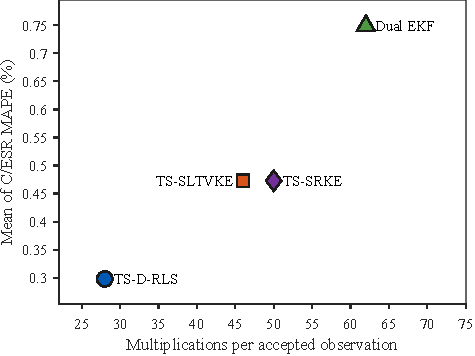
\includegraphics{fig_complexity_pareto.pdf}
\caption{共同运算计数模型下的精度--复杂度权衡。纵轴为C与ESR MAPE的算术平均，仅作Pareto可视化摘要，不作为估计器遴选目标。}
\label{fig:complexity_pareto}
\end{figure}

\section{F28379D器件级可行性}
\label{sec:device}

器件级研究检验内部ADC架构能否在寄存器可实现的时序与显式高共模模拟前端下采集所提观测。四个同步的16位差分ADC模块使用320~ns孔径，每模块维持1.093~MS/s。单边沿调度在$0.5~\mu$s保护带之后、$T_{w,R}=2.2~\mu$s内于重构边沿两侧各放置三个采样点。在所仿真的共模范围内ADC直连不可行，因此可行性以下列条件为前提：指定的差分AFE、边沿频带共模抑制比（CMRR）下界、外部基准与时钟、以及有界的标定残差。

七个代表性条件、每条件200个Monte Carlo种子，给出最坏p95容值与ESR误差$1.6425\%$与$2.6109\%$；每个条件都满足其预声明阈值。表~\ref{tab:f28379d}汇总可行性主张的证据。寄存器时序、孔径裕量、直接存储器访问流量、占用率、AFE元件假设、共模极值与覆盖范围保留在补充说明S1。

\begin{table}[t]
\caption{F28379D器件级摘要}
\label{tab:f28379d}
\centering
\begin{tabular}{ll}
\toprule
项目 & 指定值 \\
\midrule
ADC架构 & 四模块，16位差分 \\
孔径/速率 & 320~ns / 每模块1.093~MS/s \\
边沿采集 & $0.5~\mu$s保护带；$T_{w,R}=2.2~\mu$s；每侧3点 \\
AFE边界 & 差分通路；边沿频带CMRR $\ge70$~dB \\
健康报告 & 1024周期（20.48~ms） \\
最坏p95 C/ESR & $1.6425\%$ / $2.6109\%$ \\
\bottomrule
\end{tabular}
\end{table}

$1.36~\mu$s的\TSRLS{}时间是估计器算术估计值，不是平台WCET。固件编译、链接器布局、实测执行时间与台架AFE验证仍待完成；该结果支持的是受约束的仿真架构，而非硬件验证。

\section{讨论}
\label{sec:discussion}

\subsection{观测设计为何重要}

O0--O1因子分解把观测设计与估计器复杂度分离：在RLS核不变的情况下，O1按第\ref{sec:results}节报告的倍数同时降低两个MAPE与收敛时间。这一归因与电路物理一致：开关边沿暴露ESR压降，状态内电荷平衡暴露逆电容。更精巧的递推无法可靠补偿混叠这些效应或比较错位时间戳的观测。

在范围界定的文献矩阵中，没有已公开方法同时组合\Cuk{}传递电容对象、$+i_{L1}\leftrightarrow-i_{L2}$换流、时间戳重构边沿信息与方向专属电荷/边沿更新。这是有边界的综述发现，不是普适的文献首创主张。

\subsection{为何\TSSRKE{}为主、\TSRLS{}保留什么}

\TSSRKE{}满足全部四条预声明主判据：在每个静态、噪声/时序与工作瞬态行上与其Kalman母体逐位一致（真实健康变化之外监督器零触发），保持母体$88.93\%$的同时覆盖率（接近$\approx90.25\%$的独立性基准），并在远小于一个报告间隔的时间内整定突变健康阶跃——母体冻结之处，RLS基线则需长一个数量级的时间。监督器因此以每行4次额外乘法消除了有校准实现的唯一失格性失效。该选择不意味着普适优越：\TSRLS{}保留最低静态ESR误差、最快原生收敛、全部时长上更优的斜坡跟踪汇总与最低成本，在只需平滑退化点跟踪的场合仍是推荐实现。Dual EKF因不带门控而更快整定ESR阶跃，但其未校准覆盖率与最差虚假ESR瞬态使其仍被排除。两个保留实现因此互补——\TSRLS{}是轻量的实用估计器，\TSSRKE{}是感知不确定度的突变恢复扩展。第\ref{sec:results}节的最小监督闭环校验显示：调节器瞬态下监督器零误触发，反馈下突变以亚毫秒级恢复。

\subsection{局限}

证据有七条主要边界。
\begin{enumerate}
\item 可辨识性与更新要求有效CCM；DCM与弱激励区间保持估计，可用性已在第\ref{sec:results}节向轻载边界量化。方法假设两个电感电流均可测；缺少任一测量的应用需要附加传感器或经独立验证的电流重构。
\item 所报告的ESR是在建模的开关、热与频率条件下的有效状态指标，不是与温度无关的老化变量。在实际部署中，温度引起的ESR变化可能超过本文报告的辨识误差；健康趋势判断因此要求热工况匹配的比较或到参考温度$r_C(T_{\mathrm{ref}})$的映射，而这超出本工作的仿真范围。
\item $0.1$--$100$~s轨迹是合成或轨迹推导的带宽测试，不是运行至失效的数据；突变不连续是恢复压力测试而非老化事件。
\item 边沿振铃、隔离/探头、AFE共模抑制与量产标定的硬件验证仍待完成。
\item F28379D研究是器件级仿真；目标编译与实测WCET尚未演示。
\item 监督器解决了原跟踪--置信权衡中的突变恢复一侧，但\TSRLS{}对平滑斜坡的跟踪仍更好，辅助的\TSRLS{}区间仍覆盖不足；监督器组件是经典的，其常数虽经预声明并在全部案例共享，但设计时面向的是所评估的扰动类别。
\item 闭环与轻载补充使用Model-A对象、每案例单噪声种子与一个刻意简化的PI调节器；监督闭环校验共享这些限制。它们不评估控制器交互广度或DCM模式运行。
\end{enumerate}

\subsection{实验路线图}

下一阶段应在能量传递支路中使用受控C/ESR网络、指定的F28379D调度、分离的绝对/边沿电压通路与同步电感电流测量。测试应扫掠输入电压、占空比、负载与温度；表征振铃与AFE抑制；对照离线阻抗测量验证标定；并在固件发布前实测WCET。

\section{结论}
\label{sec:conclusion}

本文把\Cuk{}变换器正常的双向能量传递转化为两个拓扑同步的电容健康观测——ESR的时间戳重构开关边沿行与容值的ESR补偿安全窗电荷行——并证明了在有效CCM门控下建立C--ESR局部可辨识性的正有限窗信息下界。在这些观测之上，监督重置估计器\TSSRKE{}弥合了无监督核的跟踪--置信缺口：它在稳态与其Kalman母体完全一致、同时区间覆盖率$88.93\%$接近名义值，并在母体冻结之处以$1.52$与$0.48$~ms整定突变容值与ESR阶跃，代价是每行4次额外乘法。

在盲矩阵上，把通用混合观测换成所提观测集，在RLS核不变的情况下将容值MAPE从$7.0366\%$降到$0.3727\%$——承载最大增益的是观测设计而非估计器复杂度。\TSSRKE{}随后取得$0.3011\%/0.6446\%$的C/ESR MAPE，而轻量\TSRLS{}基线保留最佳静态ESR误差、斜坡跟踪与成本，在只需平滑退化点跟踪的场合仍被推荐。补充研究在闭环调节下保持了管线精度、量化了到轻载边界的可用性，并使噪声驱动误差在投运配置处保持在条件噪声CRLB的小倍数以内；受约束的F28379D仿真以最坏p95误差$1.6425\%/2.6109\%$支持器件级可行性。

在实验或寿命主张成立之前，硬件与加速老化研究仍须验证AFE共模行为、振铃、温度依赖性、标定迁移与实测执行时间。

\appendix

\section{所采用符号约定下的开关方程}
\label{app:equations}

为完整起见，用于验证观测符号的一阶开关方程保留传递电容ESR，其余寄生量置零。这里$v_C$为理想电容电压，$v_T=v_C+r_Ci_C$。当$u=1$（主开关导通）时，
\begin{align}
\dot i_1&=V_{\mathrm{in}}/L_1, &
\dot i_2&=(v_C-r_Ci_2-v_o)/L_2,\\
\dot v_C&=-i_2/C, &
\dot v_o&=i_2/C_o-v_o/(RC_o).
\end{align}
当$u=0$（主开关关断）时，
\begin{align}
\dot i_1&=(V_{\mathrm{in}}-v_C-r_Ci_1)/L_1, &
\dot i_2&=-v_o/L_2,\\
\dot v_C&=i_1/C, &
\dot v_o&=i_2/C_o-v_o/(RC_o).
\end{align}
这些方程蕴含式~\eqref{eq:ic_unified}，并在Model-A的可选电感、开关、二极管与源寄生量置零后与其指定实现一致。ESR符号在两个状态间不同，因为$u=0$时$i_C=+i_1$而$u=1$时$i_C=-i_2$。

\section{标量协方差包络}
\label{app:covariance}

设有限窗起点的后验标量方差为$P_n$。过程累积给出$P_n^-\le P_n+Q_N$。同化总标量信息$\mu$，得
\begin{equation}
P_{n+1}\le\left(\frac{1}{P_n+Q_N}+\mu\right)^{-1},
\end{equation}
即式~\eqref{eq:cov_recursion}。令$P_{n+1}=P_n=P^*$，得
\begin{equation}
\mu(P^*)^2+\mu Q_NP^*-Q_N=0,
\end{equation}
其正根即式~\eqref{eq:fixed_point}。该映射递增且上界为$1/\mu$。当$Q_N=0$时取逆得$P_{n+1}^{-1}\ge P_n^{-1}+\mu$，故$P_n\le(P_0^{-1}+n\mu)^{-1}$。在有界条件失配下，须加入有限的、依案例的误差项。

经验证的最大不动点为归一化容值方向的$0.0112191$与ESR方向的$8.82437\times10^{-6}$。

\bibliographystyle{IEEEtran}
\bibliography{references}

\end{document}
